\documentclass{article}
\usepackage{graphicx} % Required for inserting images
\usepackage{hyperref}
\usepackage{tcolorbox}

\title{Assignment 4 Computation Creativity}
\author{Batch size of 3}
\date{November 2023}

\begin{document}

\maketitle

% 1. a clear description of the algorithm, architecture, parameter choices, and tuning process. What code did you use/have to write? How long did it take to train? What was your input/training data? What problems did you encounter and overcome? What did you learn that you would tell another student trying to do the same thing?

% 2. results and critical discussion. Are the images/videos reasonable? What are some notable success and failure cases?

% 3. ethical implications. Yes, you may have made something fun and cool, but what are the ethical implications of the software you used? Could the same approach be used for the purposes of misinformation/harm? 

\section{LoRA}
Low Rank Approximation [1] is a way to fine tune a base model without having to train all of the weights again. By training two smaller matrices that can be much smaller (rank), the fine-tuning can be much faster and the size of the model itself is significantly smaller. This was originally developed for large language models but cloneofsimo on \href{https://github.com/cloneofsimo/lora}{Github} was the first to adapt it to be used for diffusion models.

\subsection{Algorithm, Implementation \& Usage}
For the training of LoRA, kohya-ss's scripts are used through a WebUI (\href{https://github.com/bmaltais/kohya_ss}{Github} to fine-tune the LoRA. The type of LoRA that was used in the repo was "LoRA-LierLa: LoRA for Linear layers and Conv2d layers with a 1x1 kernel"; there isn't a paper for this specific type anywhere that we could find.

\subsubsection{Setting Up the Repo}
We followed along with this \href{https://rentry.org/ezlora}{guide} to setup the repo and do the training. We also used Ubuntu 22.04 and Python 3.10.6 for this since the repo recommends using Python 3.10.
\begin{verbatim}
    git clone https://github.com/bmaltais/kohya_ss.git
    cd kohya_ss
    python -m venv venv
    source ./venv/bin/activate
    bash setup.sh
    accelerate config
\end{verbatim}

\newpage
Setting up the accelerate config:
\begin{verbatim}
    This machine
    No distributed training
    No (CPU only)
    No (torch dynamo)
    No (DeepSeed)
    1 (GPU ID) (I had two GPUs so either 0 or 1)
    BF16 (precision) (30XX and 40XX RTX cards should use BF16)
\end{verbatim}
Run the GUI with:
\begin{verbatim}
    bash gui.sh
\end{verbatim}

\subsubsection{Preparing Data}
Professor Radke allowed us to train a LoRA with his likeness and graciously provided us with pre-cropped 512x512 images of himself.
\begin{center}
    \includegraphics[scale=0.125]{.imgs/dataset/00000-0-P3095395.jpg}
    \includegraphics[scale=0.125]{.imgs/dataset/00003-0-PXL_20221009_180554011.jpg}
    \includegraphics[scale=0.125]{.imgs/dataset/00007-0-PXL_20230204_202340837.MP.jpg}
    \includegraphics[scale=0.125]{.imgs/dataset/00008-0-PXL_20230218_175154938.MP.jpg} \\
    Examples of the dataset
\end{center}

We manually create text files for each image describing the scene in the corresponding image. Most of them were just "radke, short hair, smiling, looking at viewer". We realize afterwards that we should have described the scene in natural language ("Radke looking at the viewer smiling") instead of tags because the original Stable Diffusion model was trained on natural language and realistic images. This was due to the fact that we were used to the NovelAI model, in which was trained on anime images and used tags separated by commas.
\begin{center}
    \includegraphics[scale=1.0]{.imgs/other/tagging.png} \\
    Example of "tagging" an image
\end{center}

We put in the images in a directory "imgs/55\_radke\_lora\_v1.5\_(2)" where 55 is obtained from 1000 divided by number of images $(1000/18\approx 55)$.

\newpage
Next download the we downloaded a config json (\href{https://pastebin.com/dl/ZgbbrE7f}{https://pastebin.com/dl/ZgbbrE7f}) and save it in the folder. It contains the config for training LoRA's.

\begin{verbatim}
{
  "pretrained_model_name_or_path": "runwayml/stable-diffusion-v1-5",
  "v2": false,
  "v_parameterization": false,
  "logging_dir": "",
  "train_data_dir": "",
  "reg_data_dir": "",
  "output_dir": "",
  "max_resolution": "512,512",
  "learning_rate": "0.0001",
  "lr_scheduler": "constant",
  "lr_warmup": "0",
  "train_batch_size": 1,
  "epoch": 3,
  "save_every_n_epochs": 1,
  "mixed_precision": "fp16",
  "save_precision": "fp16",
  "seed": "58008",
  "num_cpu_threads_per_process": 2,
  "cache_latents": true,
  "caption_extension": "",
  "enable_bucket": true,
  "gradient_checkpointing": false,
  "full_fp16": false,
  "no_token_padding": false,
  "stop_text_encoder_training": 0,
  "xformers": true,
  "save_model_as": "safetensors",
  "shuffle_caption": true,
  "save_state": false,
  "resume": "",
  "prior_loss_weight": 1.0,
  "text_encoder_lr": "1e-4",
  "unet_lr": "0.0001",
  "network_dim": 128,
  "lora_network_weights": "",
  "color_aug": false,
  "flip_aug": false,
  "clip_skip": 2,
  "gradient_accumulation_steps": 1.0,
  "mem_eff_attn": false,
  "output_name": "last",
  "model_list": "runwayml/stable-diffusion-v1-5",
  "max_token_length": "150",
  "max_train_epochs": "",
  "max_data_loader_n_workers": "",
  "network_alpha": 128,
  "training_comment": "",
  "keep_tokens": "0",
  "lr_scheduler_num_cycles": "",
  "lr_scheduler_power": "",
  "persistent_data_loader_workers": false,
  "bucket_no_upscale": true,
  "random_crop": false,
  "bucket_reso_steps": 64.0,
  "caption_dropout_every_n_epochs": 0.0,
  "caption_dropout_rate": 0,
  "optimizer": "AdamW8bit",
  "optimizer_args": "",
  "noise_offset": "",
  "LoRA_type": "Standard",
  "conv_dim": 1,
  "conv_alpha": 1,
  "sample_every_n_steps": 0,
  "sample_every_n_epochs": 0,
  "sample_sampler": "euler_a",
  "sample_prompts": "",
  "additional_parameters": ""
}
\end{verbatim}

\noindent Go to the LoRA tab and load the above config in the WebUI.

\subsubsection{Training the LoRA}
We need to change the following hyperparameters:
\begin{verbatim}
    Use SD1.5 (Since we are training on a realistic subject)
    Clip Skip = 1 (Again realistic subject)
    Mixed Precision = BF16 (30xx or 40xx card)
    Save Precision = FP16 (ALWAYS MAKE SURE ITS FP16)
    Sample Epochs = 1 (You can do steps also if preferred)
\end{verbatim}
The rest of the hyperparameters in the config were left unchanged.

\newpage


\subsection{Results}
Training this LoRA on 18 images for 3 epochs on one 4090 took 5 minutes.

\noindent Here are some results with different sampling steps and samplers:
\begin{center}
    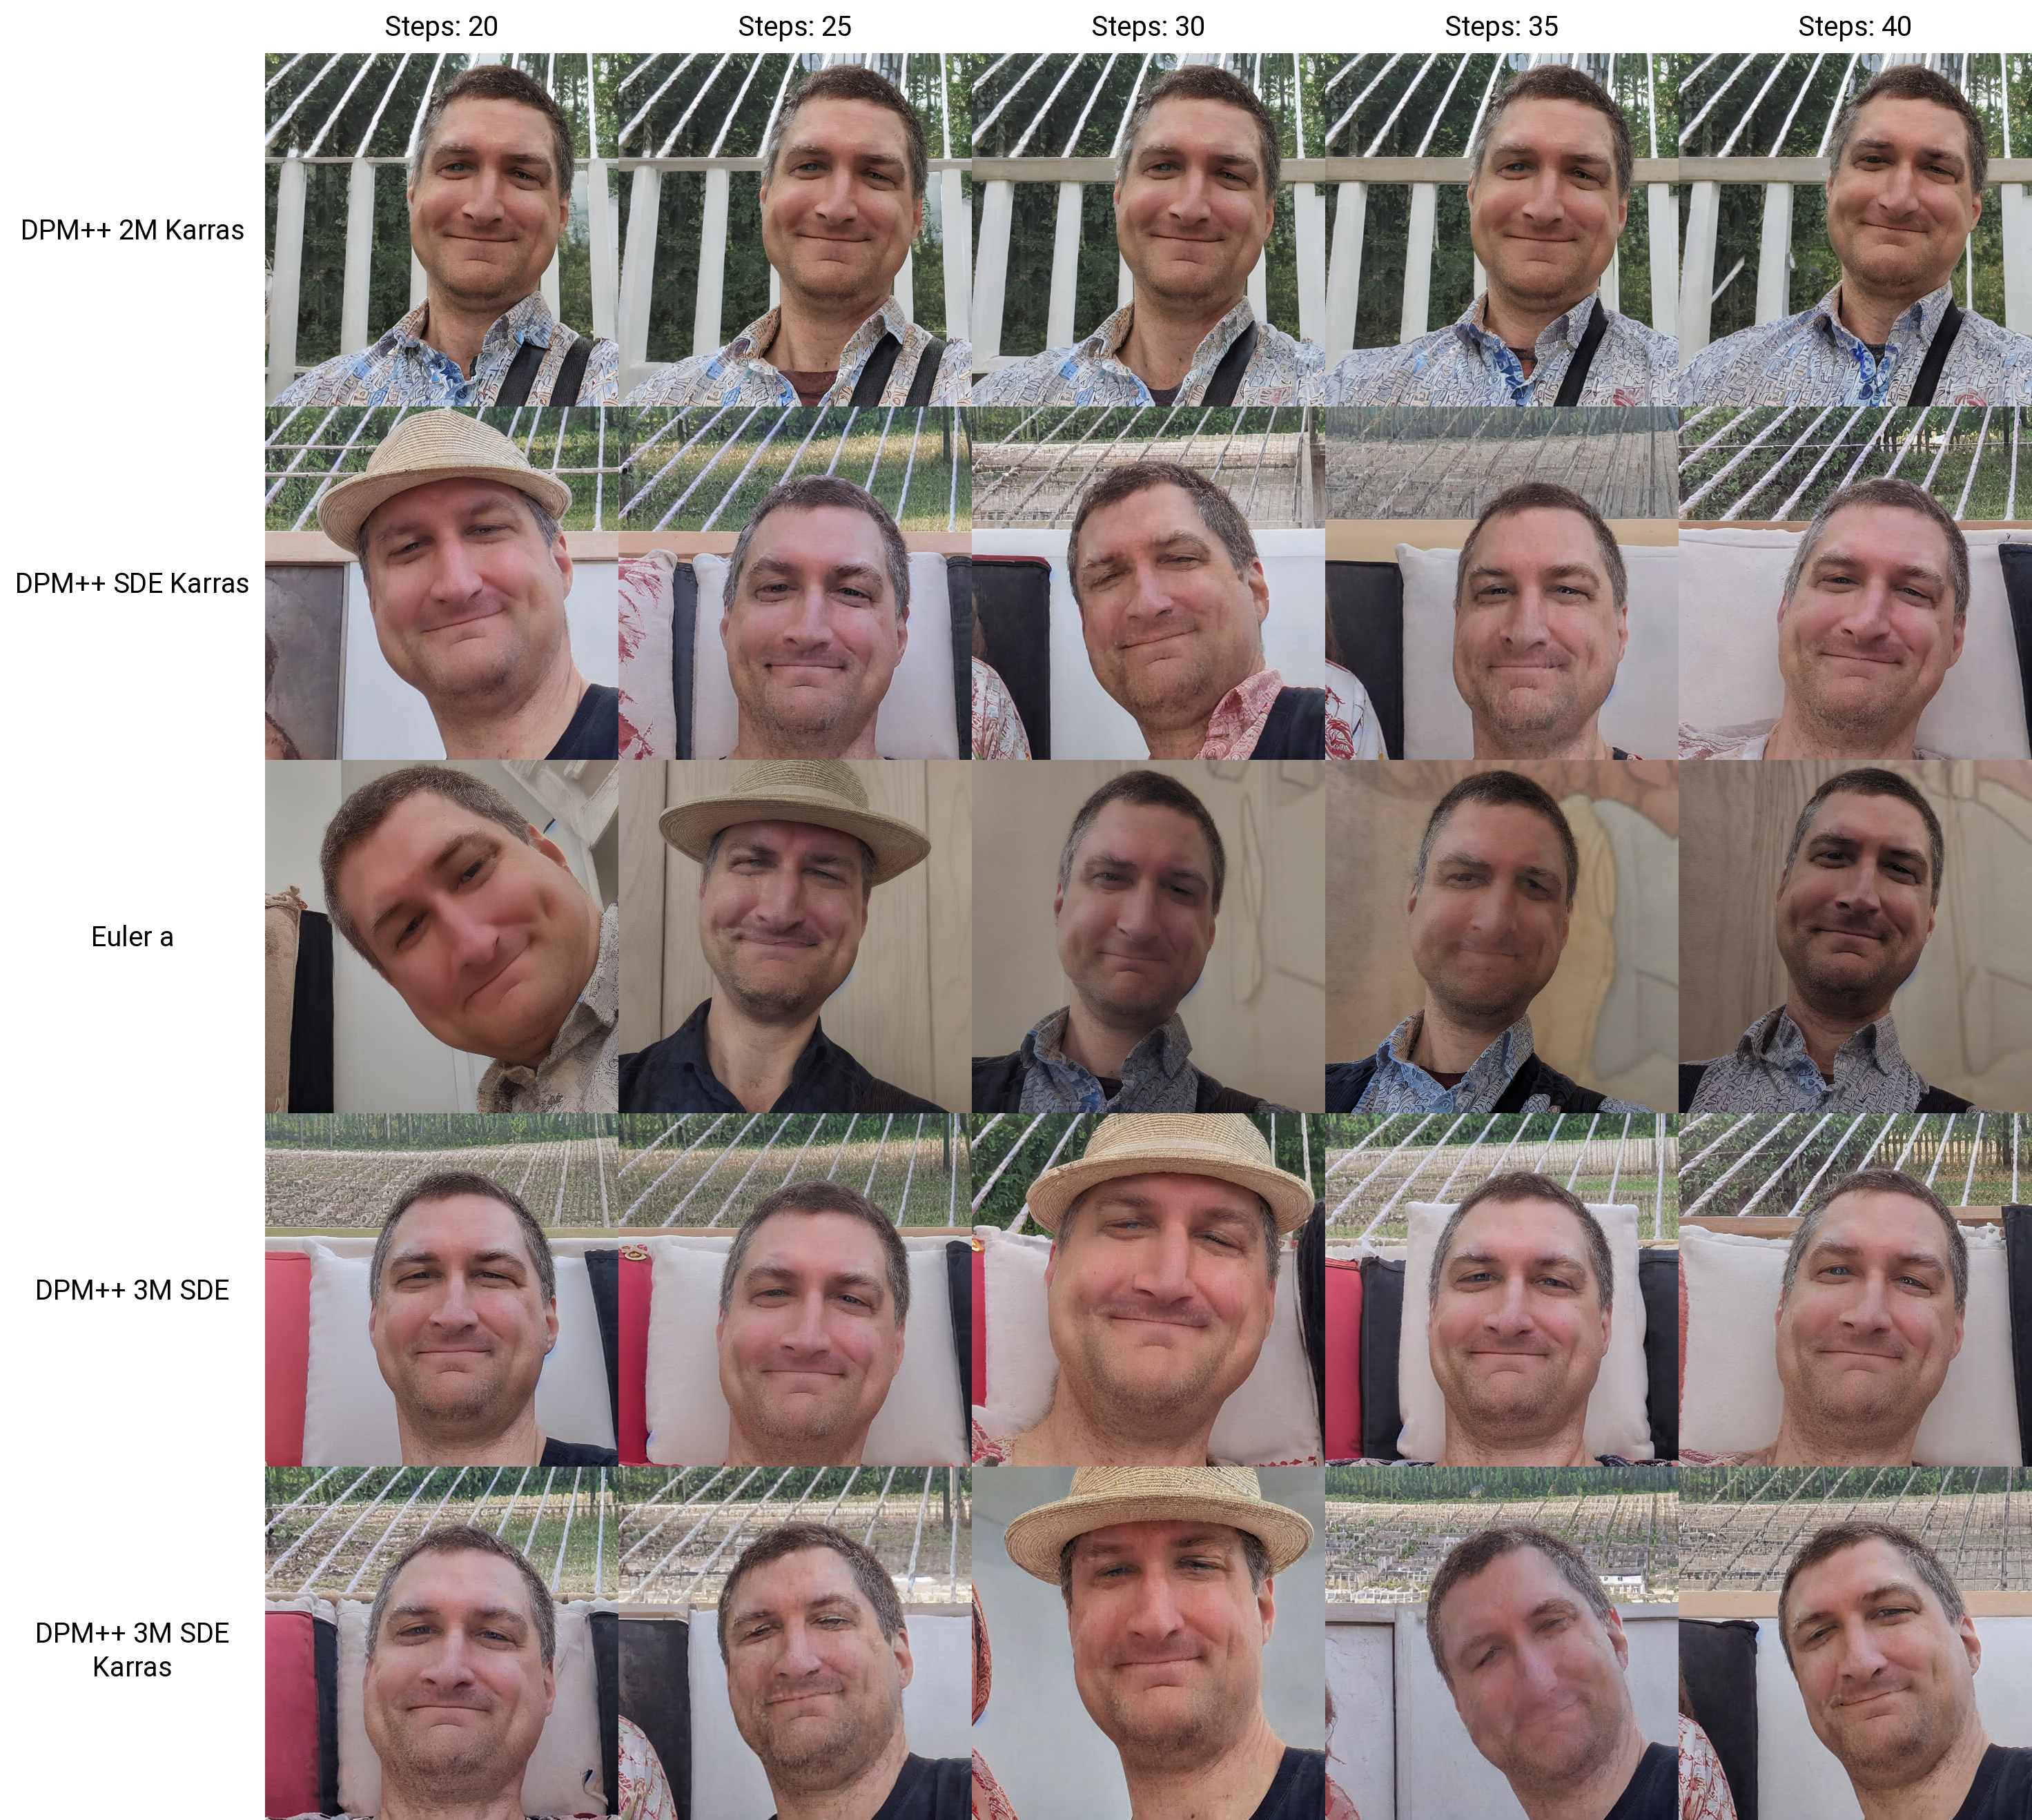
\includegraphics[scale=0.1]{.imgs/radke_lora_v1.5_(2)_prompting_2.png} \\
    Generated with the same seed
\end{center}
We can see that the model has learned what Prof. Radke looks like however the model seems to have overfit on the training data as seen on the following image. The model learned that Radke's hammock and pillows along with his face for this seed.
\begin{center}
    \includegraphics[scale=0.2]{.imgs/radke_overfitting_2.jpg} \\
    One of the training images
\end{center}

\newpage
\noindent Here is another example:
\begin{center}
    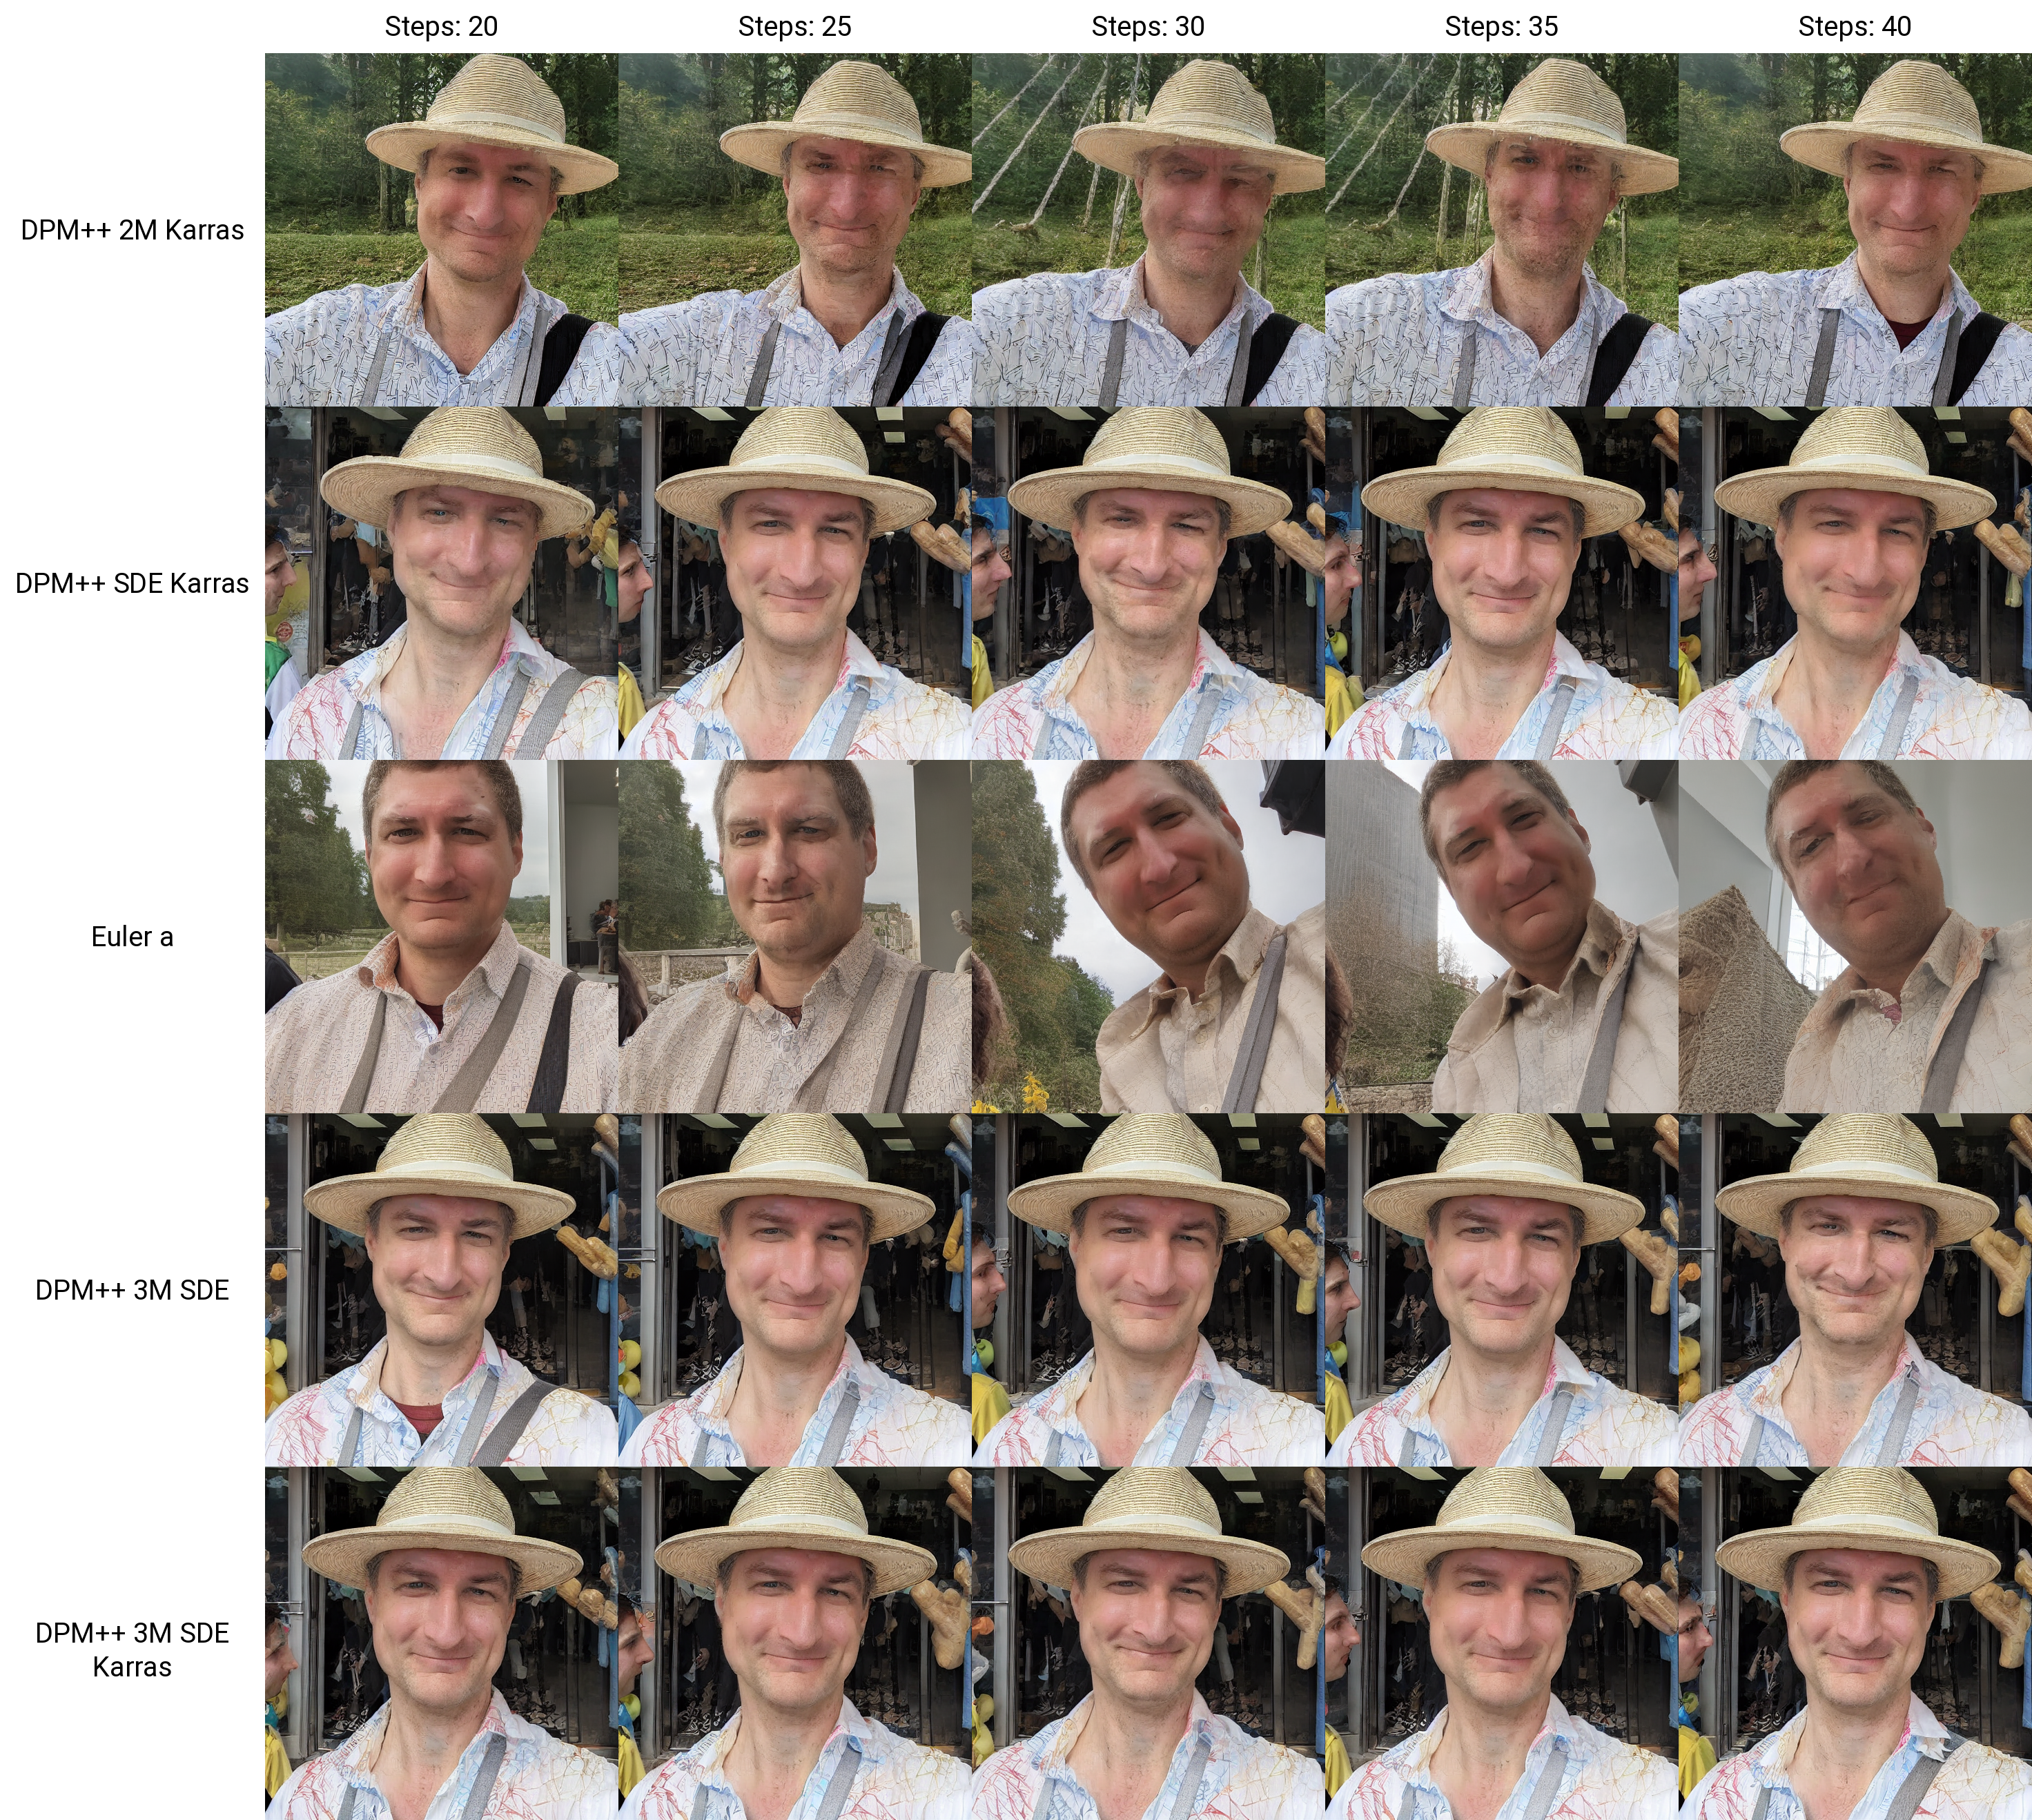
\includegraphics[scale=0.1]{.imgs/radke_lora_v1.5_(2)_prompting_3.png} \\
    Generated with the same seed
\end{center}
Again, the model seems to have overfit on the training data as seen on the following image. The model learned that Radke's hat, shirt, and the storefront that he is standing in front of.
\begin{center}
    \includegraphics[scale=0.2]{.imgs/radke_overfitting_3.jpg} \\
    One of the training images
\end{center}

\newpage
One unique difference that we realized is that for DPM++ 3M SDE, at step 20, the image generated is relatively the same as the training images. However, if we compare the two images, notice that a red shirt appears! If we examine the dataset again, note that the one of the training images has a dark red shirt along with a similar dress shirt.
\begin{center}
    \includegraphics[scale=0.35]{.imgs/radkeredshirt.PNG}
    \includegraphics[scale=0.2]{.imgs/dataset/00014-0-PXL_20230509_204242326.PORTRAIT.jpg}\\
    Generated Image (Left) with red shirt from image (Right)
\end{center}


\subsection{Ethics}
One of the greatest AI ethic conversations we have today is privacy. In class, we have delved into many intricacies of the privacy of machine learning. In one case, we described how we can use bias to define a classifier in the dataset imagenet. In a way this reflects off from how we can use personal information to the benefit of the people who have access to models. This implication is reflective of bias in classifiers like imagenet. We can set a bias for a particular dataset, which can be damaging. For instance, if I label the dataset as alcoholics for a generation, then the model will imply off that dataset, and claim that the person it trained from is an alcoholic. 

In our case, we have a dataset given to us to use of a specific person, and then we are able to apply that model to particular environments. Then, we also describe the dataset by inserting textual descriptions of what we imagine the image is in a human form. This allows us to generate images of that particular person with success in the form of that general image dataset. So, the images are only those that have a similar degree to each other. 

Although the results are not particularly amazing to the standards of generation compared to our current outlook, we can generalize the efforts in ethical proportions. Given that we have this dataset, we have to consider the fact that the dataset can still be used in a way to harm the subject even with their permission. As we mentioned previously, we can import the data and generalize fake or malicious labels in order to train an "evil" model. Or possibly develop a model in order to impersonate someone (will be more indepth for Control Net). Moreover, by placing a person in where they do not belong, it can be classified as impersonating.

In our reflection of our creations, we can always agree to the fact that it is used in a creative and fun way. However, with the idea that an existing person can be used through generation, there are many implications such as impersonation and malicious labeling. Thus, even with consent, there are many ethical factors that must be considered.

\clearpage

\section{ControlNet}

\subsection{Algorithm, Implementation \& Usage}
ControlNet$^{[2]}$ is a fine tuned version of existing diffusion models to provide more controllable image to image generations. It uses a variety of image processing techniques to extract information and features from sample images and conditions the generated image to mimic those in the sample image. The list of features extracted are as follows: Canny edge, Hough line, Scribble drawing, HED edge, Pose detections, Segmentation maps, Depth maps, Cartoon line drawing,and Normal maps.  \\ \\
The process of training ControlNet is as follows: two copies of a diffusion model is created, with one copy frozen such that the weights may not be altered. The decoder component of the trainable copy is replaced with weights of zero and fed into the frozen diffusion model at the same layers. An additional 1x1 convolutional layer is also added at the top of the trainable copy. By creating a separate training copy, this architecture minimizes overfitting when the dataset is small. Additionally, half of the training labels are removed to help the model extract semantics from the sample image alone. The full architecture is illustrated below: \\
\begin{center}
    \includegraphics[scale=0.29]{controlnet-with-stable-diffusion.png} \\
    {ControlNet Architecture \href{https://learnopencv.com/controlnet/}{https://learnopencv.com/controlnet/}}
\end{center}
This method makes it much easier to train and it is possible to do so on just high end consumer GPUs.

For our implementation, we first had an extension for ControlNet for stable diffusion webgui: \href{https://github.com/Mikubill/sd-webui-controlnet}{ControlNet extension}. Then we utilize a ControlNet model that has been specifically trained for openpose and imported it into 'models/ControlNet', \href{https://huggingface.co/lllyasviel/ControlNet-v1-1/tree/69fc48b9cbd98661f6d0288dc59b59a5ccb32a6b}{the model}. For ControlNet, OpenPose is a model in which a specific pose is derived from an image. This can be integrated with ControlNet in order to generate images with a high importance on poses.\\

Here is an example of utilizing OpenPose for our use case. We generate an image without the Radke LoRA. Then we take that image and preprocess a pose for that image. Finally, we generate the final result with an input and the pose. For example, we generated an image of a person playing basketball, then a pose is created from that image, and we input the image with the pose and a text input with LoRA.
\begin{center}
    \includegraphics[scale=0.2]{.imgs/basketball_base.png}
    \includegraphics[scale=0.2]{.imgs/basketball_pose.png}
    \includegraphics[scale=0.2]{.imgs/radke_lora_v1.5_(2)_prompting_basketball_1.png}\\
    Prompt for the general image: \verb|a man playing basketball| \\
    Prompt for the Radke image: \verb|<lora:last:1> radke playing basketball|
\end{center}

\newpage
\subsection{Results}

Here are some results generated with ControlNet openpose with different sampling steps and samplers:
\subsubsection{Radke Skateboarding}
\begin{center}
    \includegraphics[scale=0.3]{.imgs/skateboard_base.png}
    \includegraphics[scale=0.3]{.imgs/radke_lora_v1.5_(2)_prompting_skateboard_2.png}\\
    \verb|<lora:last:1> radke riding a skateboard|
    \verb|Left: Sample image              Right: With Radke LoRA|
\end{center}
OpenPose managed to capture the pose and generate an image where the limbs follow the original image and the face and hair looks very similar to Prof. Radke's face. It also interpreted the pose differently than the original image and generated an image where the skateboard is in the air.
\subsubsection{Radke In a Band as a Guitarist}
\begin{center}
    \includegraphics[scale=0.3]{.imgs/guitar_base.png}
    \includegraphics[scale=0.3]{.imgs/radke_lora_v1.5_(2)_prompting_guitar_1.png}
    \verb|<lora:last:0.9> radke in a band as a guitarist with really short hair|
    \verb|Left: Sample image              Right: With Radke LoRA|
\end{center}
For this example it managed to generate an image of someone that looks like Prof. Radke although with longer hair in the same correct pose. It did a really good job at generating the hands.

\subsubsection{Radke in a Band as a Drummer}
\begin{center}
    \includegraphics[scale=0.3]{.imgs/drummer_base.png}
    \includegraphics[scale=0.3]{.imgs/radke_lora_v1.5_(2)_prompting_drummer_1.png} \\
    \includegraphics[scale=0.3]{.imgs/drummer_base.png}
    \includegraphics[scale=0.3]{.imgs/radke_lora_v1.5_(2)_prompting_drummer_2.png} \\
    \verb|<lora:last:0.9> radke in a band as a drummer|
    \verb|Left: Sample image              Right: With Radke LoRA|
\end{center}

As you can tell, we generated the prompt separately to no success with this prompt. In both examples it seems as if the person is being tracked and generated in the background due to OpenPose. However, the model was unable to generate drums in any of our examples. Weirdly enough, note that since the model might have overfit on our data, we have a random portrait of Radke weirdly positioned in the front of which the drums are supposed to lie.

\subsubsection{Radke Jumping into a Pool}
% i can get the name
\begin{center}
    \includegraphics[scale=0.2]{.imgs/pool_base.png} \\
    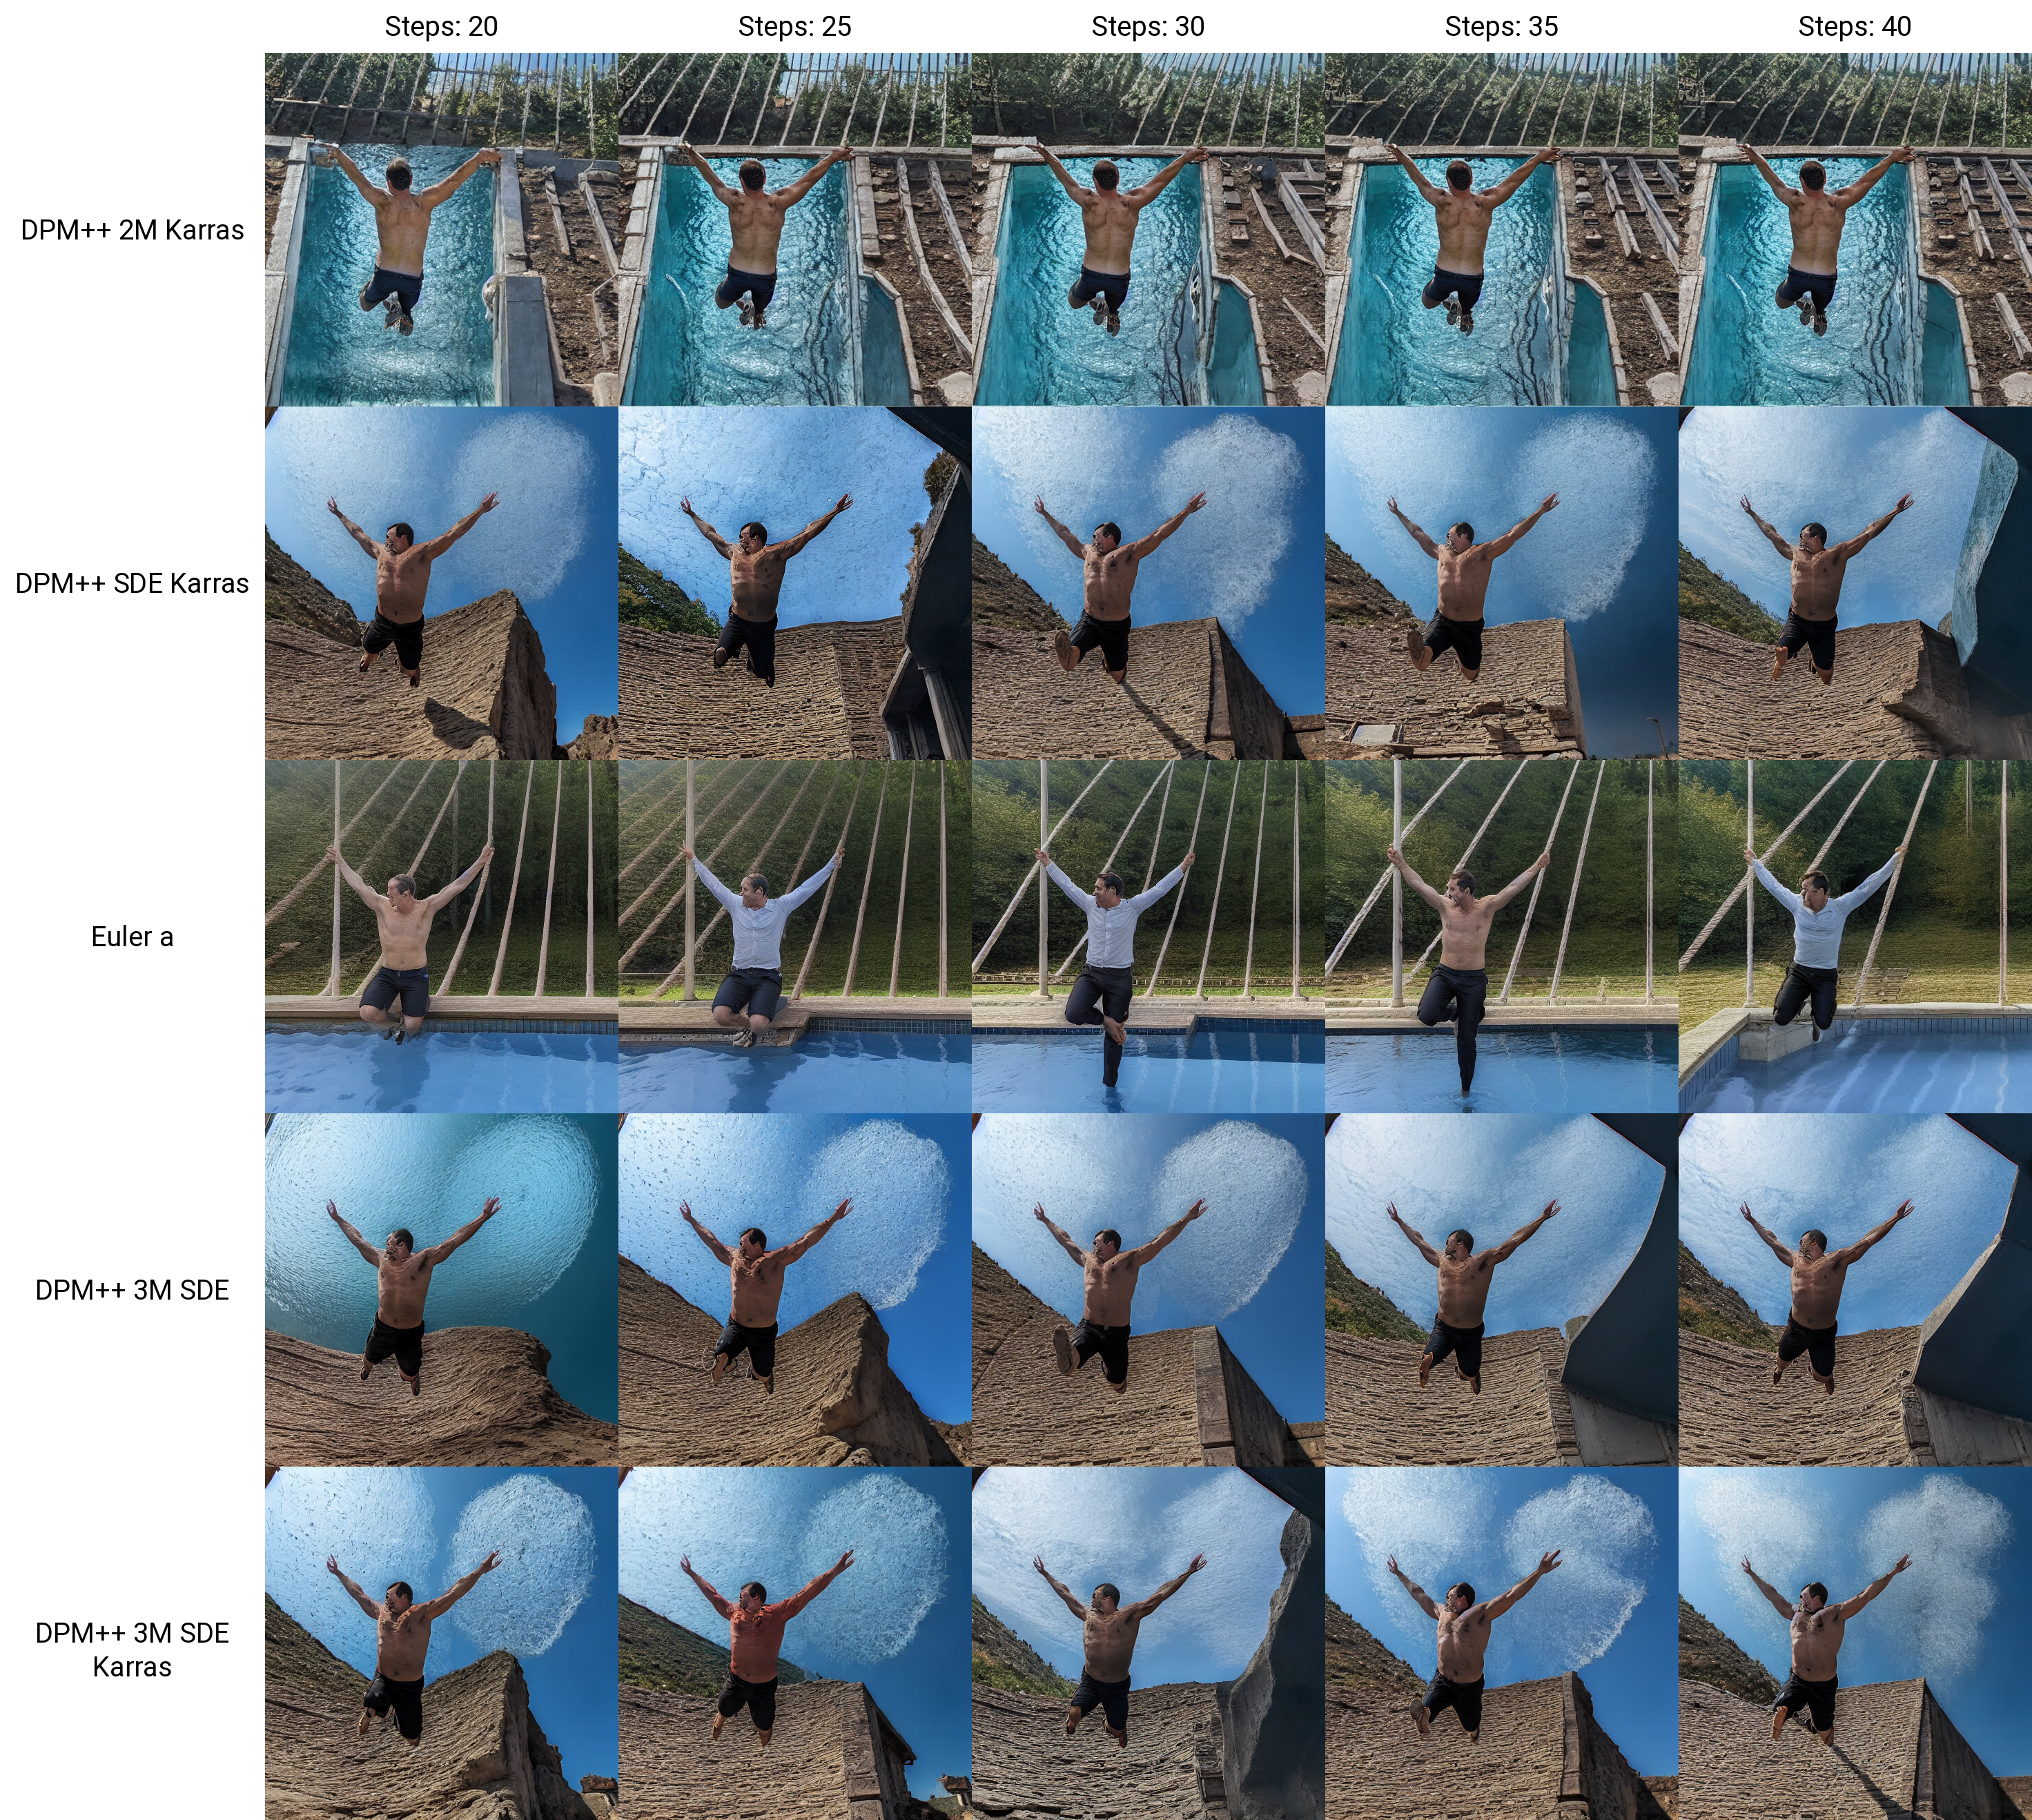
\includegraphics[scale=0.1]{.imgs/radke_lora_v1.5_(2)_prompting_pool_1.png} \\
    \verb|<lora:last:1> radke jumping into a pool|
    \verb|Top: Sample image              Bottom: With Radke LoRA|
\end{center}

If we look at one of the examples (Euler a), it is evident that the model takes a lot of inspiration from the one that has the hammock. Thus, it used that to generate ropes by the pool even though it was not relevant to what we wanted to generate. Most other samplers did not generate the pool.

% Can talk about overfitting to just portrait imgs
\newpage
\subsection{Ethics}
If we examine our results, we have some proprietary ideas of what we are able to accomplish. Which is taking our LoRA and applying it to Control Net. For instance, we are able to place a person into a generated scene with a dataset of that person. Although the results are not incredibly real or exactly definitive of the descriptions, we are able to generalize the results very well and produce an output that matches what we were looking for. In a way, this can be used to generate interesting and unique images, like a particular person jumping into the pool. However, like how we mentioned previously in LoRA, by utilizing personal information in a way where it can be used in any way, there can be malicious efforts.

For instance, impersonation is a crime in which an individual pretends to be another person in order to take advantage of a scenario where that would benefit them. This can be as small taking an exam for another person, to withdrawing funds as another person without consent. According to the New York Penal Law § 190.25: Criminal Impersonation in the Second Degree: "This offense occurs when a person pretends to be someone else with the intent to obtain a benefit or to defraud or injure another person. It is classified as a class A misdemeanor, which can carry a sentence of up to one year in jail, probation, or a fine." We can imagine that having a person pretend to be someone else can majorly impact someone in a way. Then, if we consider the methods in which we develop our model, we can impersonate others. 

In our dataset, we were able to obtain consent of Prof. Radke, and use his images to generate results for this class. However, we can use images to defraud him, perhaps transform the image in a way where we can use that in an ID. In more recent news, deep-fakes have been brought up with both voice and image generations of characters. These deep-fakes have been utilized for comedic and creative efforts, like creating videos of US presidents playing video games together. However, the realistic nature of these deepfakes can be used in a malicious way to impersonate a higher authority. Control Net and deepfakes fall into the same line of impersonation given the efforts in using them. In another consideration, what if we did not have consent of a particular person to use their imagery? If we took a dataset of a celebrity, which due to the paparazzi are very common to the internet, then we can produce images with no consent of another person.

Moreover, by generating images and placing a person specifically in a general area can be used in a creative effort to defame another individual. Thus, placing another individual at a scene or an area without them being in that position. There are multiple types of defamation that we can utilize: libel, written or displayed or slander, spoken. Since we are generating images of our target, we lie under libel. In a case of non-negligent behavior, there can be images taken out of context that can damage others. Take for example, if you are running for presidency, and your campaign solely depended on the fact that you are sober from alcohol. A generated image of you drinking alcohol can easily be a large cost against your presidential run.

All in all, in a way we provided some examples of malicious ways that generative art can be used, especially in our case where we utilize data of real people. In addition to that, we provide a case of criminality that comes with the baggage of training a model that can perform very well and used maliciously. Thus, as we get closer to models that can work very well, we get into a higher consideration of ethically of AI generation. Ergo, with great power comes great responsibility.

\section{Addendum}

\subsection{Initial Experimentation}
We originally used the \href{https://github.com/d8ahazard/sd_dreambooth_extension}{DreamBooth extension} for \href{https://github.com/AUTOMATIC1111/stable-diffusion-webui}{AUTOMATIC1111's WebuUI} for the first try of training a fine-tuned model on a specific person/character.

\subsubsection{First Experiment with Hitori Gotou from Bocchi the Rock!}
Using this \href{https://github.com/d8ahazard/sd_dreambooth_extension/wiki/ELI5-Training}{tutorial} that came with the extension, we wanted to first try fine-tuning a model with images from an anime of a character named Hitori Gotou before trying the final experiment with Prof. Radke.
\begin{center}
    \includegraphics[scale=0.15]{.imgs/dataset/chrome_1DyVxJTRDj.jpg}
    \includegraphics[scale=0.15]{.imgs/dataset/chrome_9AQfr0PW0g.jpg}
    \includegraphics[scale=0.15]{.imgs/dataset/chrome_mwcqZdCXfv.jpg} \\
    Example images from training set
\end{center}

We used a pre-trained SD1.5 model: \href{https://civitai.com/models/24779?modelVersionId=93208}{Dark Sushi Mix}, which is specifically trained on anime styled images as our base model: Our trials were not very good for either DreamBooth or LoRA fine-tuning:
\begin{center}
    \includegraphics[scale=0.2]{.imgs/bocchi_(1)_5220.png}
    \includegraphics[scale=0.2]{.imgs/bocchi_lora_(2)_2160.png} \\
    Dreambooth and LoRA Results
\end{center}

\newpage
\subsubsection{Second Experiment with Prof. Radke}
We wanted to try using SD2.1 instead of SD1.5 for this fine-tuning but while fine-tuning the model, the sample generations only generated this brown image and nothing else.
\begin{center}
    \includegraphics[scale=0.2]{.imgs/radke2.1.png} \\
    Failed generation
\end{center}

We weren't sure what was causing this problem so we decided to just switch back to SD1.5. But when fine-tuning this mode, the sample generations became more corrupted over time but only on Prof. Radke's face:
\begin{center}
    \includegraphics[scale=0.2]{.imgs/radke_lora_v1.5_(1)_3400.png} \\
    Corrupted sample generation
\end{center}
However when restarting and continuing the fine-tuning process, the samples started off not corrupted but became corrupted again over time:
\begin{center}
    \includegraphics[scale=0.2]{.imgs/radke_lora_v1.5_(1)_3570.png}
    \includegraphics[scale=0.2]{.imgs/radke_lora_v1.5_(1)_9180.png} \\
    Samples from after restarting and continuing fine-tuning
\end{center}

\newpage
\subsubsection{Generating Black Images for Samples}
Throughout the fine-tuning process for all of the above models, there was a persistent problem where some of the samples generated from the fine-tuning were just all black.
\begin{center}
    \includegraphics[scale=0.2]{.imgs/bocchi_lora_(2)_4140.png}
\end{center}
The AUTOMATIC1111 WebUI help page says:
\begin{tcolorbox}
Video cards Certain GPU video cards don't support half precision: a green or black screen may appear instead of the generated pictures. Use \verb|--upcast-sampling|. This should stack with \verb|--xformers| if you are using. If still not fixed, use command line arguments \verb|--precision full --no-half| at a significant increase in VRAM usage, which may require \verb|--medvram|.
\end{tcolorbox}

Doing the suggested and adding the following to the launch parameters: \verb|--xformers --upcast-sampling --precision full --no-half|, didn't fix the bug.

\subsubsection{Loading LoRA's for txt-2-img Generation}
Usually you would put the model in your \verb|models/lora/| directory and prompt SD with \verb|<lora:NAME:S>| where S is the strength from $[0, 1]$ or just \verb|<lora:NAME>|; but doing so with didn't seem to work as seen by the following:
\begin{center}
    \includegraphics[scale=0.2]{.imgs/radke_lora_v1.5_(1)_prompting.png} \\
    Prompt: \verb|<lora:last>, radke, looking at viewer, smiling|
\end{center}
At this point, this is where we switched from using the DreamBooth extension on AUTOMATIC1111's WebUI to using kohya-ss WebUI for the results at the beginning of the paper.

\section{References}
[1] \url{https://arxiv.org/abs/2106.09685} \newline
[2] \url{https://learnopencv.com/controlnet} \\
\end{document}
